En el apartado de hardware se destaca, como bien dijimos, el uso de tres 
motores paso a paso 28BYJ-48 cuyas especificaciones son:
\begin{itemize}
  \item Tensión nominal de entre 5V y 12 V.
  \item 4 Fases.
  \item Resistencia 50 Ω.
  \item Par motor de 34 Newton / metro (aprox. 0,34 Kg por cm).
  \item Consumo de unos 55 mA.
  \item 8 pasos por vuelta.
  \item Reductora de 1 / 64.
  \item Unipolar
\end{itemize}
\begin{figure}[!htb]
  \begin{center}
    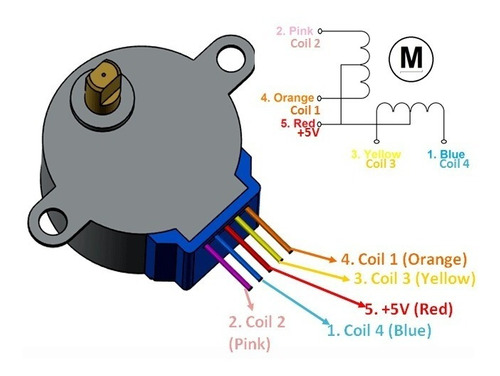
\includegraphics[width=0.4\textwidth]{imagenes/28BYJ_48.jpg}
  \end{center}
  \caption{Motor $28BYJ_48$}
  \label{fig:28BYJ_48}
\end{figure}
\FloatBarrier
Para controlar estos motores, se emplearón drives UNL2003 constituido por dos transistores en configuración Darlington.
\begin{figure}[!htb]
  \begin{center}
    \subfloat[]{{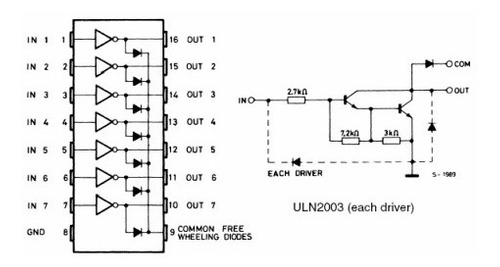
\includegraphics[width=6cm]{imagenes/ULN2003.jpg} }}%
    \qquad
    \subfloat[]{{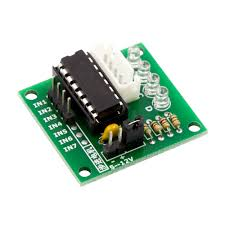
\includegraphics[width=4cm]{imagenes/ULN2003_PCB.jpg} }}%
  \end{center}
  \caption{Driver ULN2003}
  \label{fig:Driver ULN2003}
\end{figure}
\FloatBarrier
Para la apertura y cierre de la pinza, se utilizó un servo motor Sg90; el cual posee
un torque de 9 gramos.
\begin{figure}[!htb]
  \begin{center}
    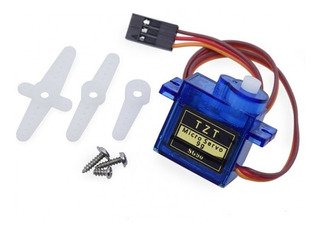
\includegraphics[width=0.4\textwidth]{imagenes/servo.jpg}
  \end{center}
  \caption{Servo Sg90}
  \label{fig:servo}
\end{figure}


